\documentclass[12pt,a4paper]{article}
\usepackage[utf8]{inputenc}
\usepackage[greek,english]{babel}
\usepackage{alphabeta} 
\usepackage[pdftex]{graphicx}
\usepackage[top=1in, bottom=1in, left=0.5in, right=0.5in]{geometry}
\linespread{1}
\setlength{\parskip}{8pt plus2pt minus2pt}
\widowpenalty 10000
\clubpenalty 10000
\newcommand{\eat}[1]{}
\newcommand{\HRule}{\rule{\linewidth}{0.5mm}}
\usepackage[official]{eurosym}
\usepackage{enumitem}
\setlist{nolistsep,noitemsep}
\usepackage[hidelinks]{hyperref}
\usepackage{cite}
\usepackage{lipsum}
\graphicspath{ {./images/} }
\usepackage{listings}
\usepackage{color}
\setlength{\parindent}{0pt}


\definecolor{dkgreen}{rgb}{0,0.6,0}
\definecolor{gray}{rgb}{0.5,0.5,0.5}
\definecolor{mauve}{rgb}{0.58,0,0.82}


\lstset{frame=tb,
	language=C,
	aboveskip=3mm,
	belowskip=3mm,
	showstringspaces=false,
	columns=flexible,
	basicstyle={\small\ttfamily},
	numbers=none,
	numberstyle=\tiny\color{gray},
	keywordstyle=\color{blue},
	commentstyle=\color{dkgreen},
	stringstyle=\color{mauve},
	breaklines=true,
	breakatwhitespace=true,
	tabsize=3
}


\title{ECE 351 Lab 9}
\author{Zachary DeLuca}
\date{March 28 2023}

\begin{document}
	
\maketitle
\hline
\section*{Introduction}
	In this lab we will plot functions along with relevant information about the function in the Fourier space. Once the function is plotted in the time domain, there will be accompanying plots that show the magnitude of their transfer function along with the phase shift they induce. As each of the frequency domain functions have values along a large domain, we will then zoom in to focus on the more relevant data. 

\section*{Results}
For this lab, we needed to do the same set of commands on different functions. The function was to plot the graphs that were spit out of the function that was given in the report. Each of the following figures accompanies the function that was sent to the frequency domain to analyze. \vspace*{12pt}

The first function we had to work with was: 
$$f(t)=cos(2\pi t)$$
\begin{center}
	\subsection*{Figure 9.1}
	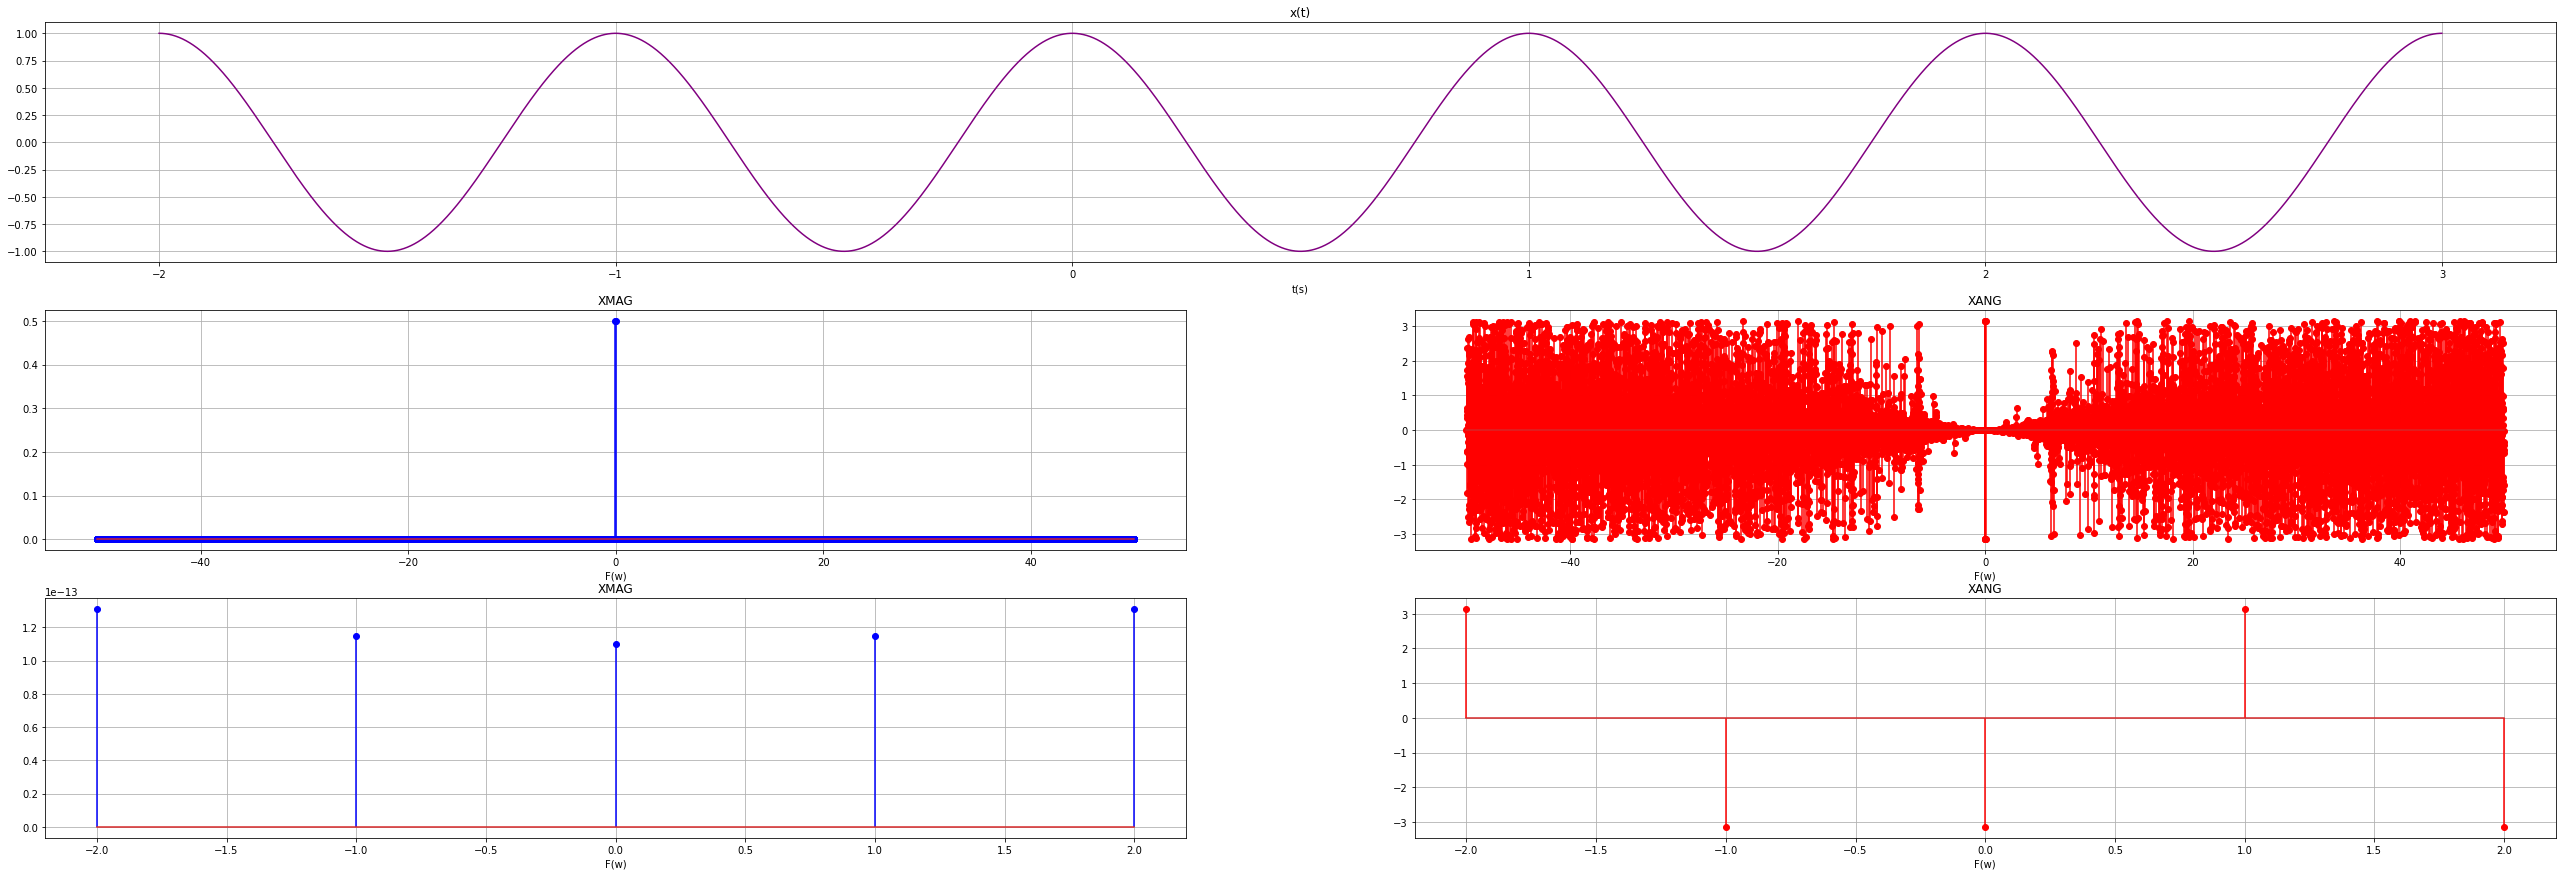
\includegraphics[width = 7in]{/home/zachariahmus/Documents/Code_Projects/ECE351/ECE351/Lab9/Figure 2023-04-06 220342.png}
\end{center}
\vspace*{12pt}

$$f(t)=5sin(2\pi t)$$
\begin{center}
	\subsection*{Figure 9.2}
	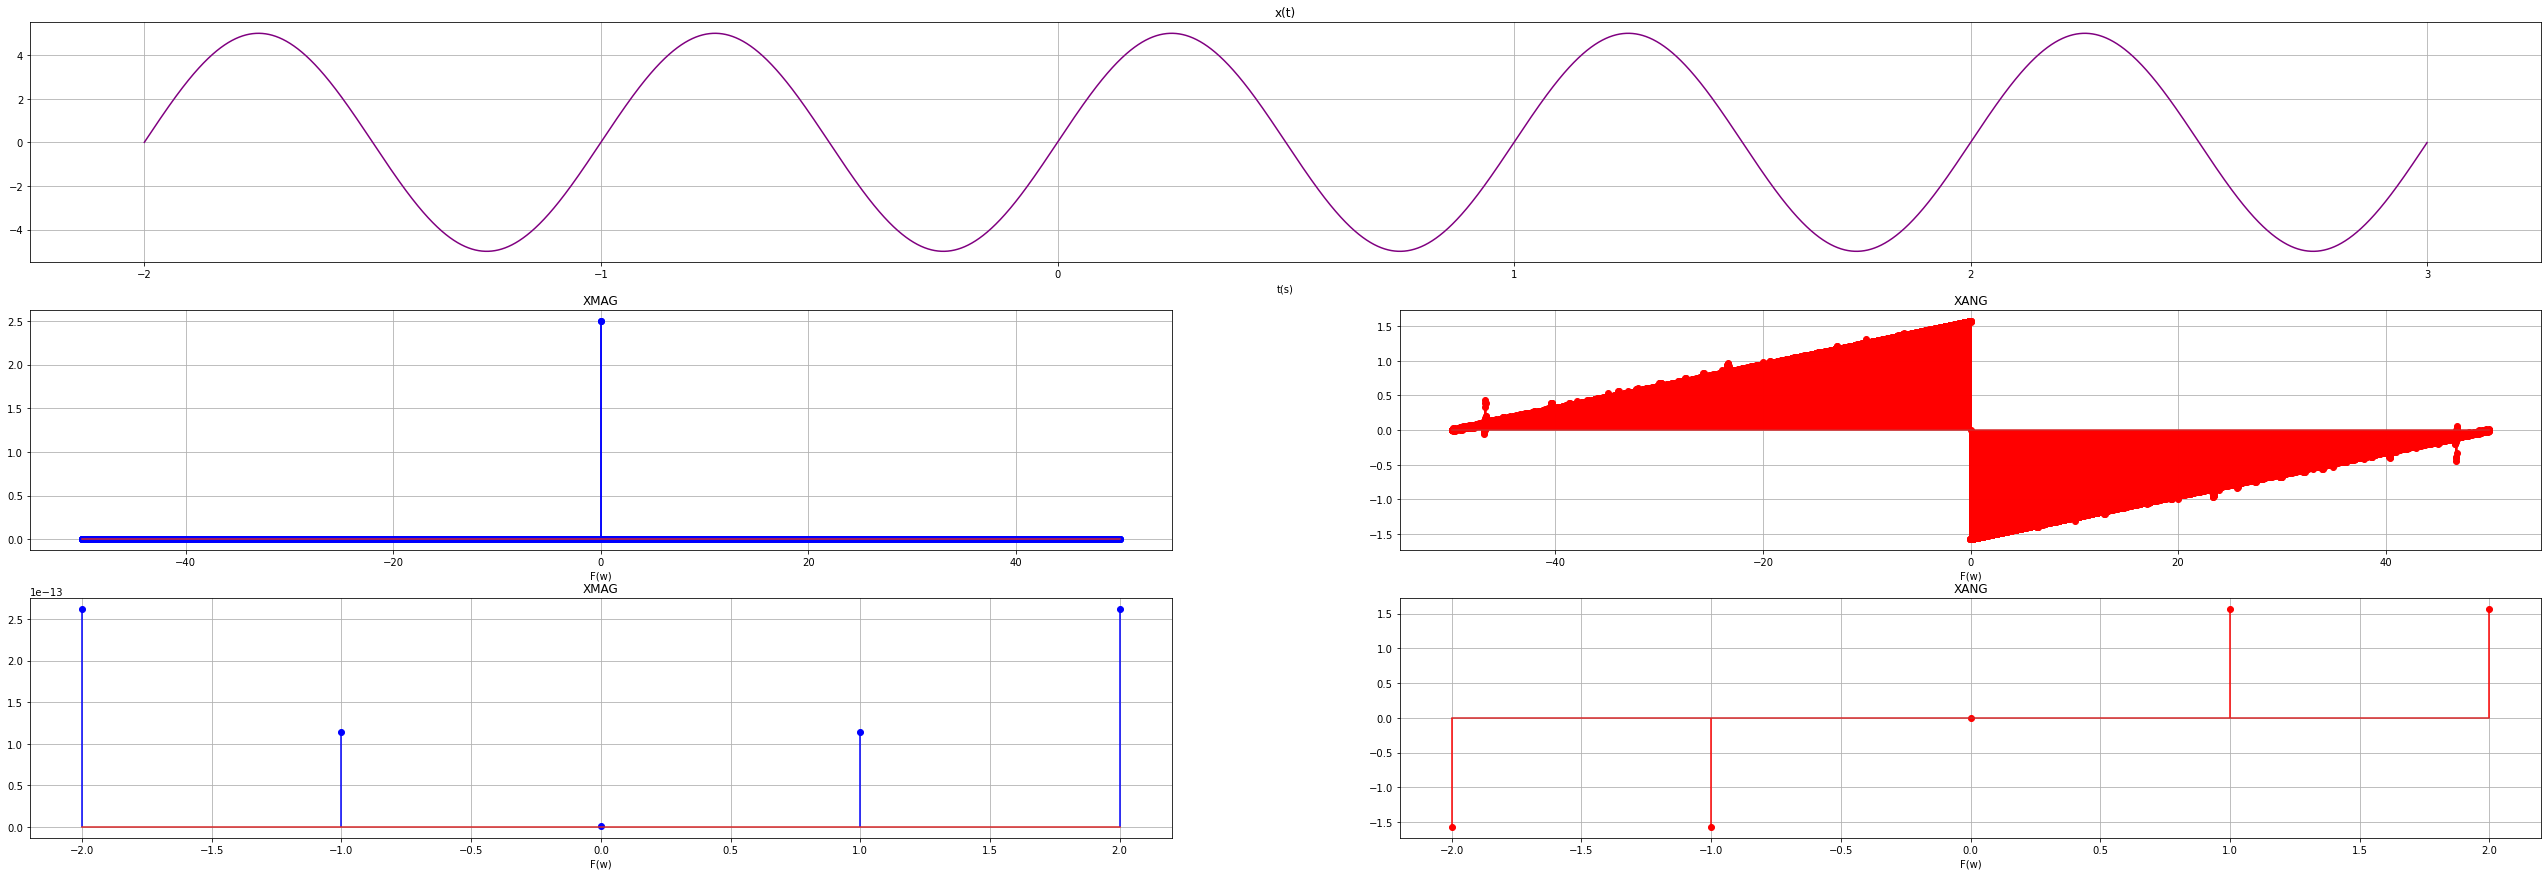
\includegraphics[width = 7in]{/home/zachariahmus/Documents/Code_Projects/ECE351/ECE351/Lab9/Figure 2023-04-06 220345.png}
\end{center}

$$2cos(4\pi t-2)+sin^2(12\pi t+3)$$
\begin{center}
	\subsection*{Figure 9.3}
	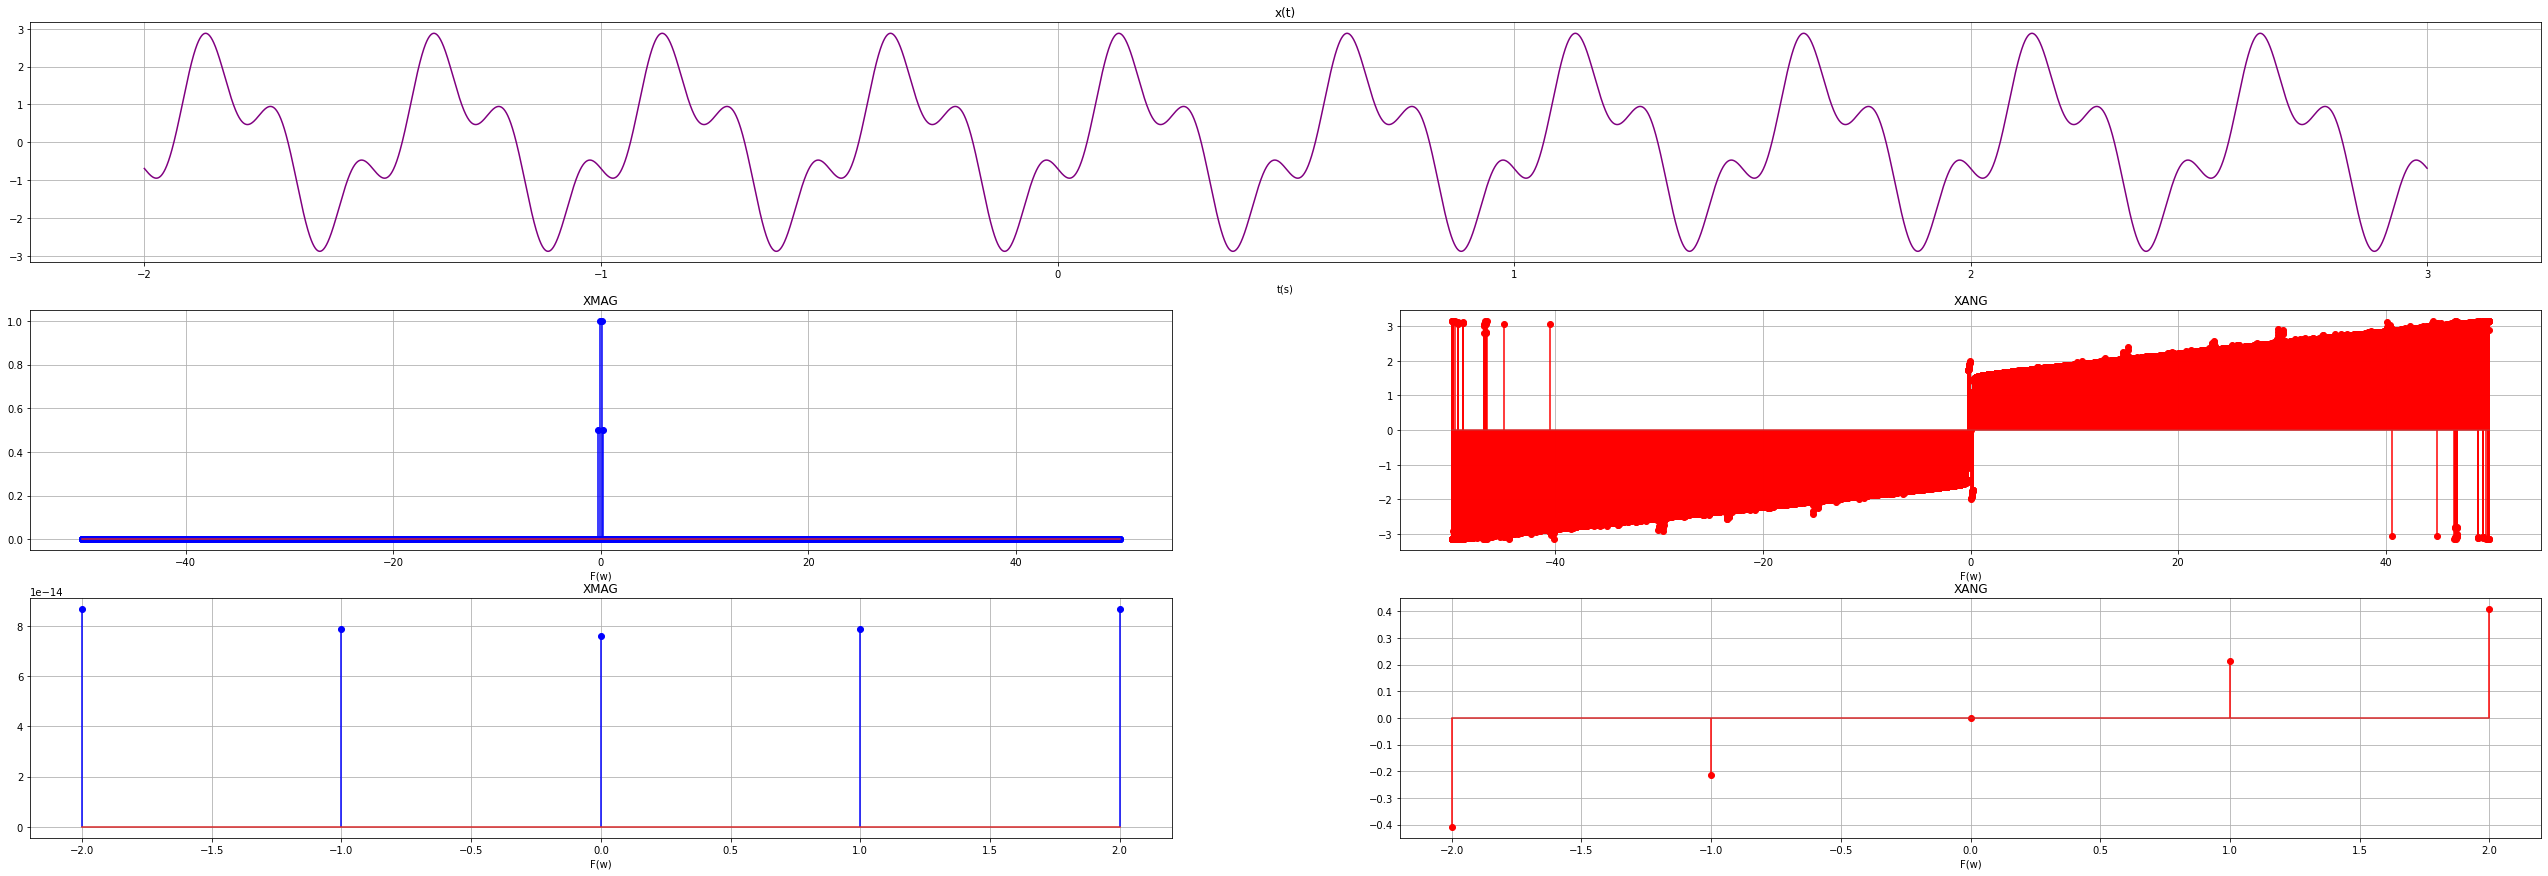
\includegraphics[width = 7in]{/home/zachariahmus/Documents/Code_Projects/ECE351/ECE351/Lab9/Figure 2023-04-06 220347.png}
\end{center}
\newpage
This last graph comes from the analysis of the Fourier series representation of a square wave as shown in lab 8. We used the N=15 approximation for this set. 
\begin{center}
	\subsection*{Figure 9.4}
	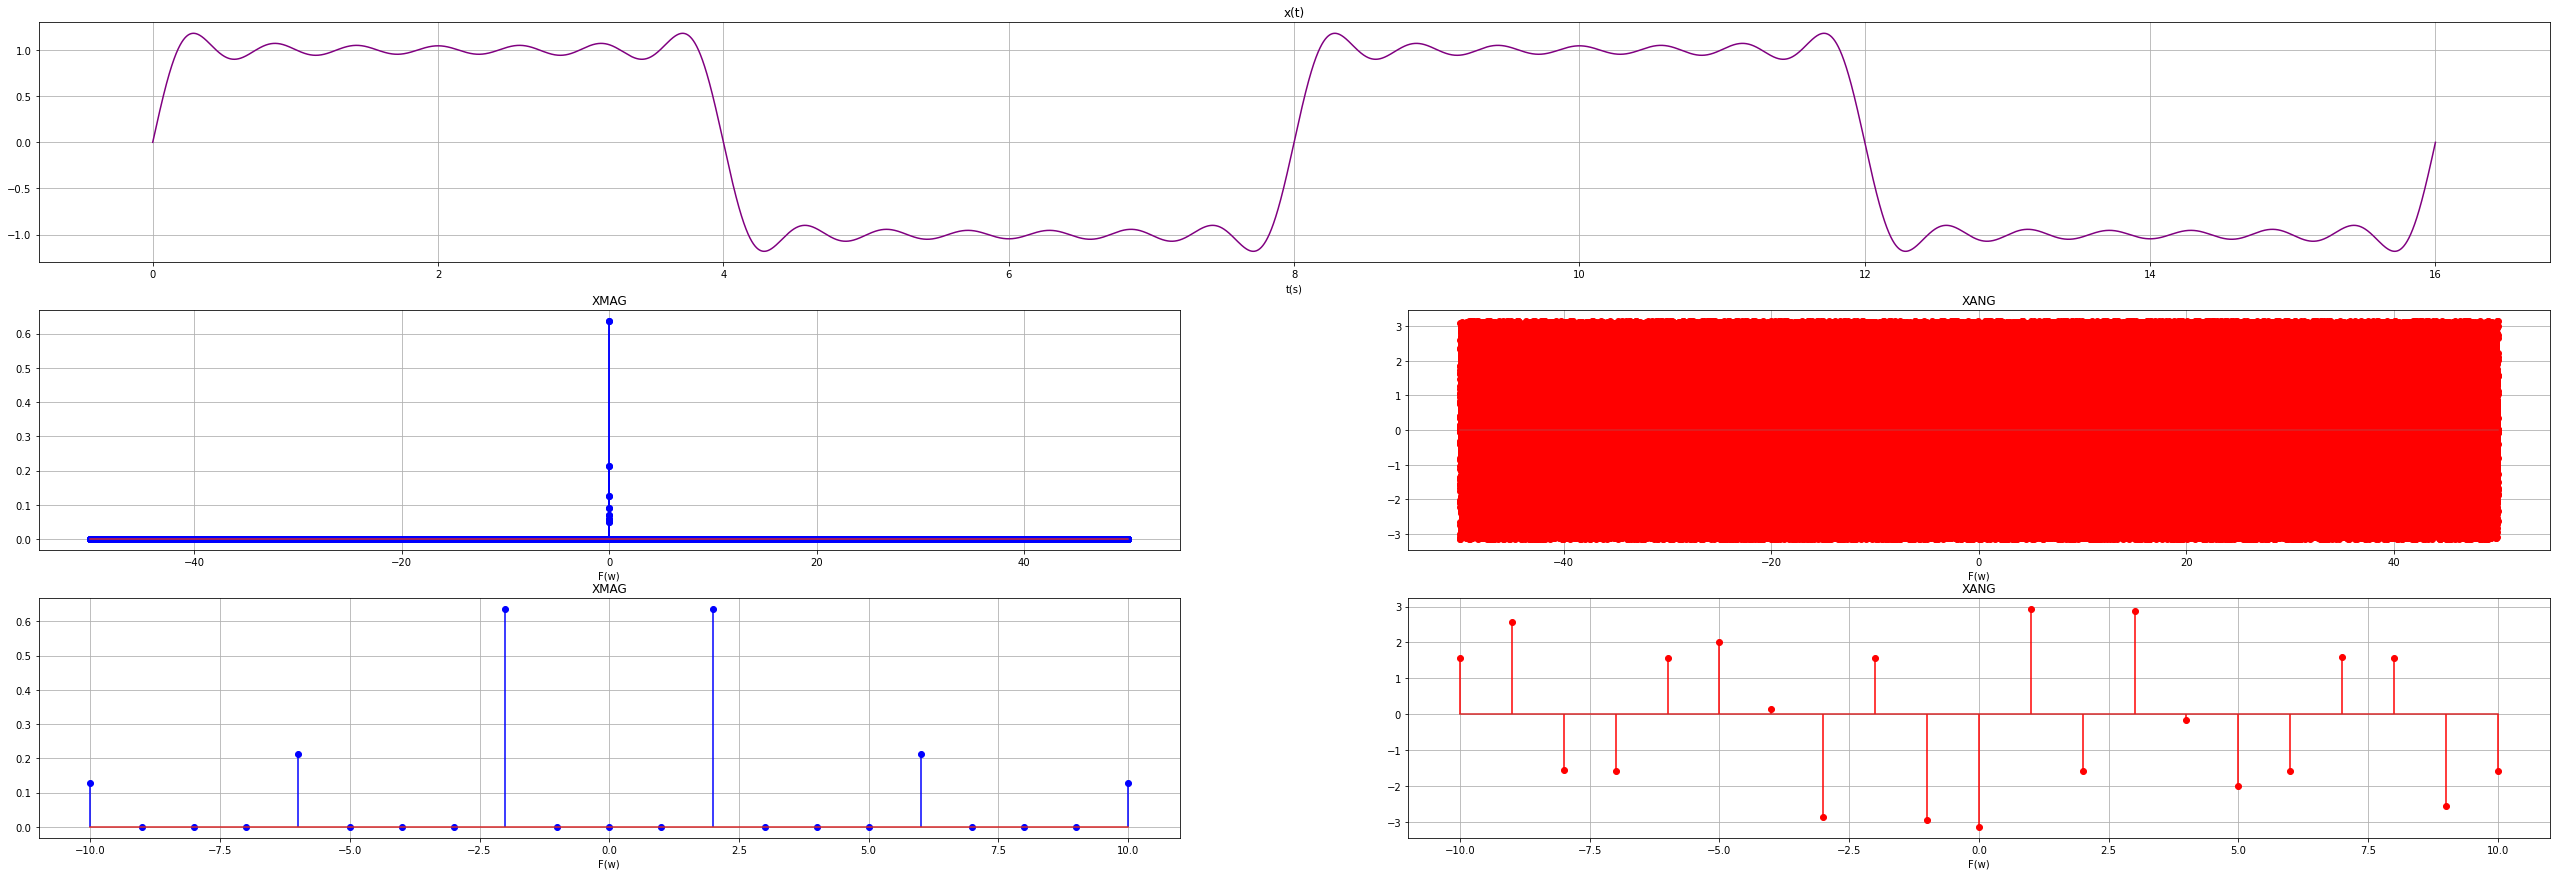
\includegraphics[width = 7in]{/home/zachariahmus/Documents/Code_Projects/ECE351/ECE351/Lab9/Figure 2023-04-06 220349.png}
\end{center}



\vspace{12pt}
	

\section*{Post Lab Questions}
1. What happens if fs is lower? If it is higher? fs in your report must span a few orders of
magnitude.\vspace*{12pt}

If the fs is lower, the x axis shrinks in the frequency domain and grows as fs grows. The axis grows as there is increased precision, not because of larger window of data, so the shape of the graph does not change. The following set has been tested to illustrate this point: 
\begin{center}
	\subsection*{fs=10}
	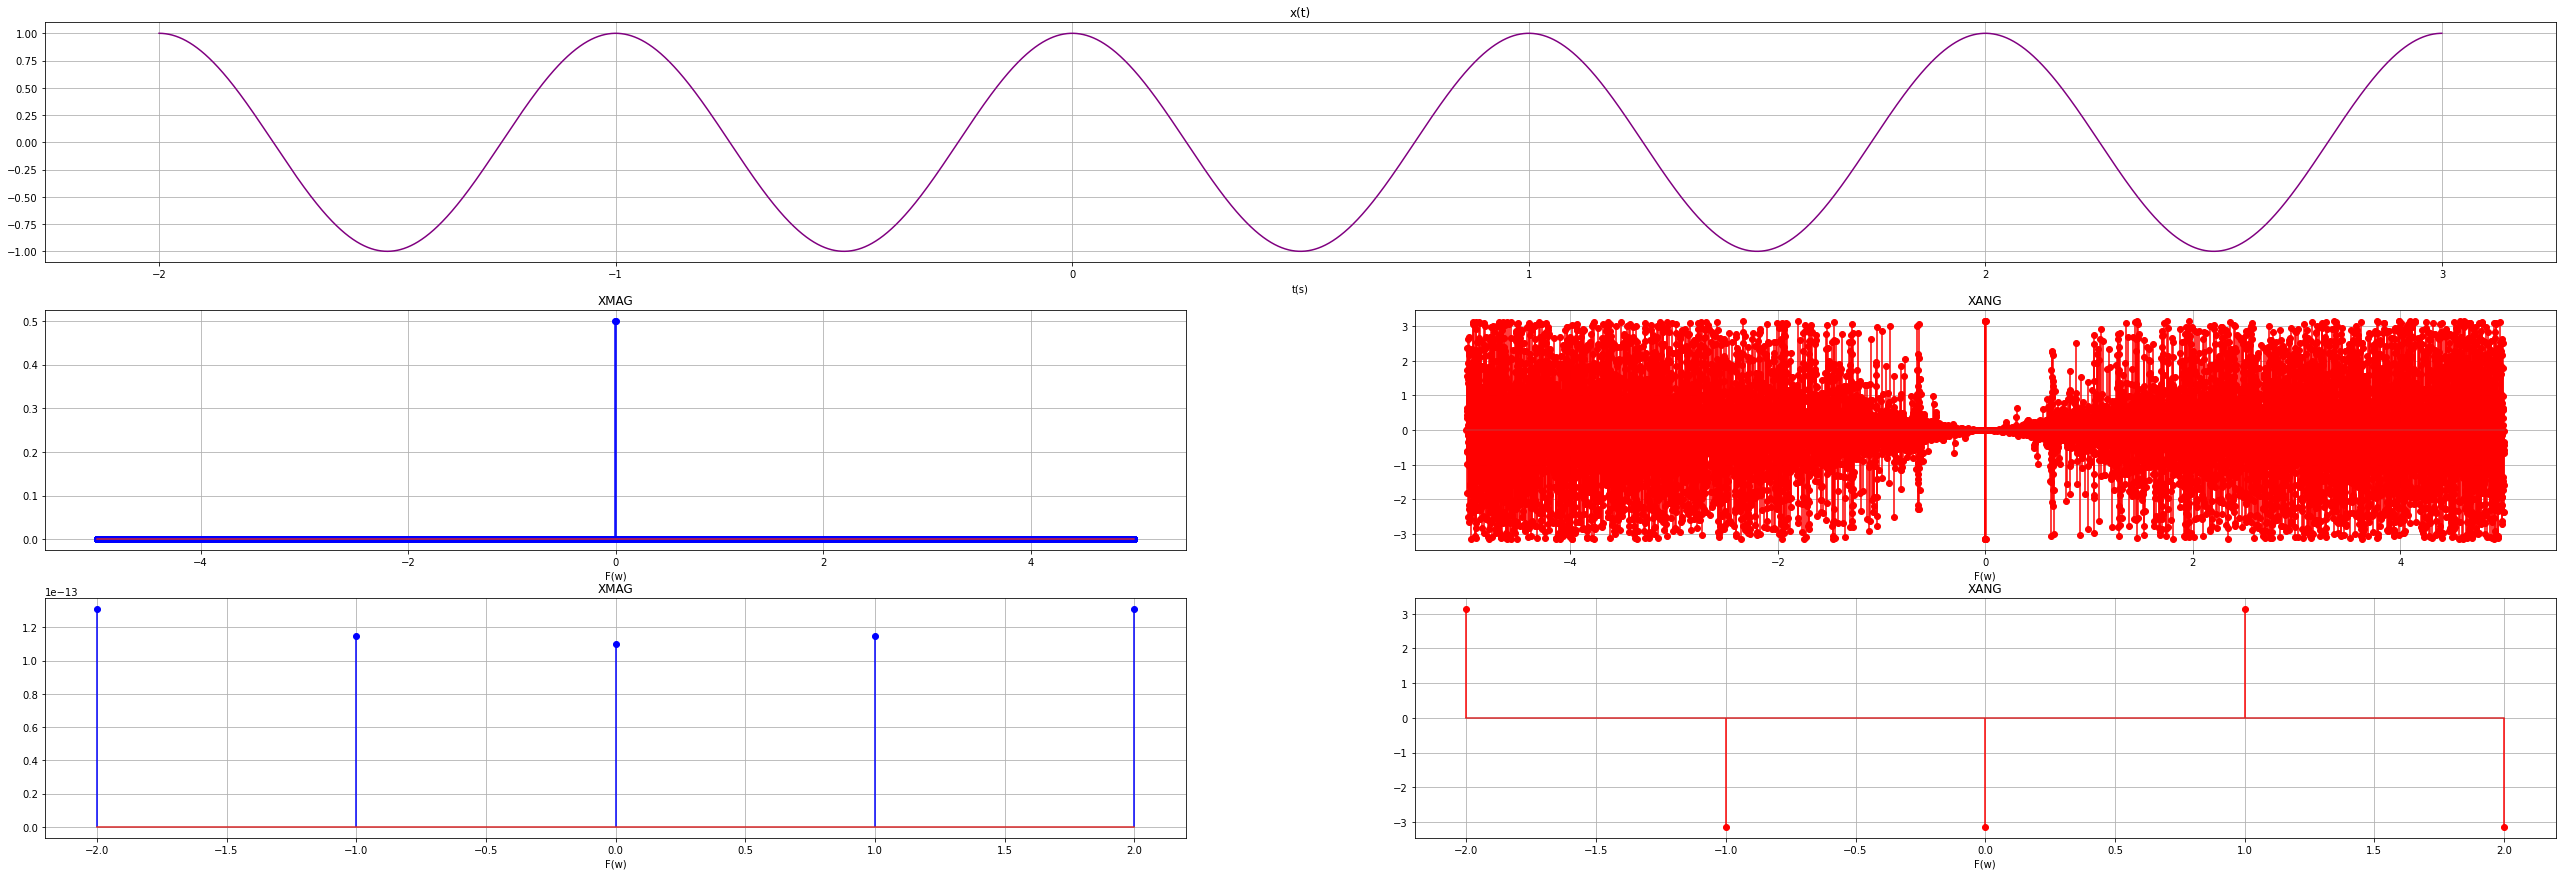
\includegraphics[width = 7in]{/home/zachariahmus/Documents/Code_Projects/ECE351/ECE351/Lab9/10.png}
\end{center}

\begin{center}
	\subsection*{fs=100}
	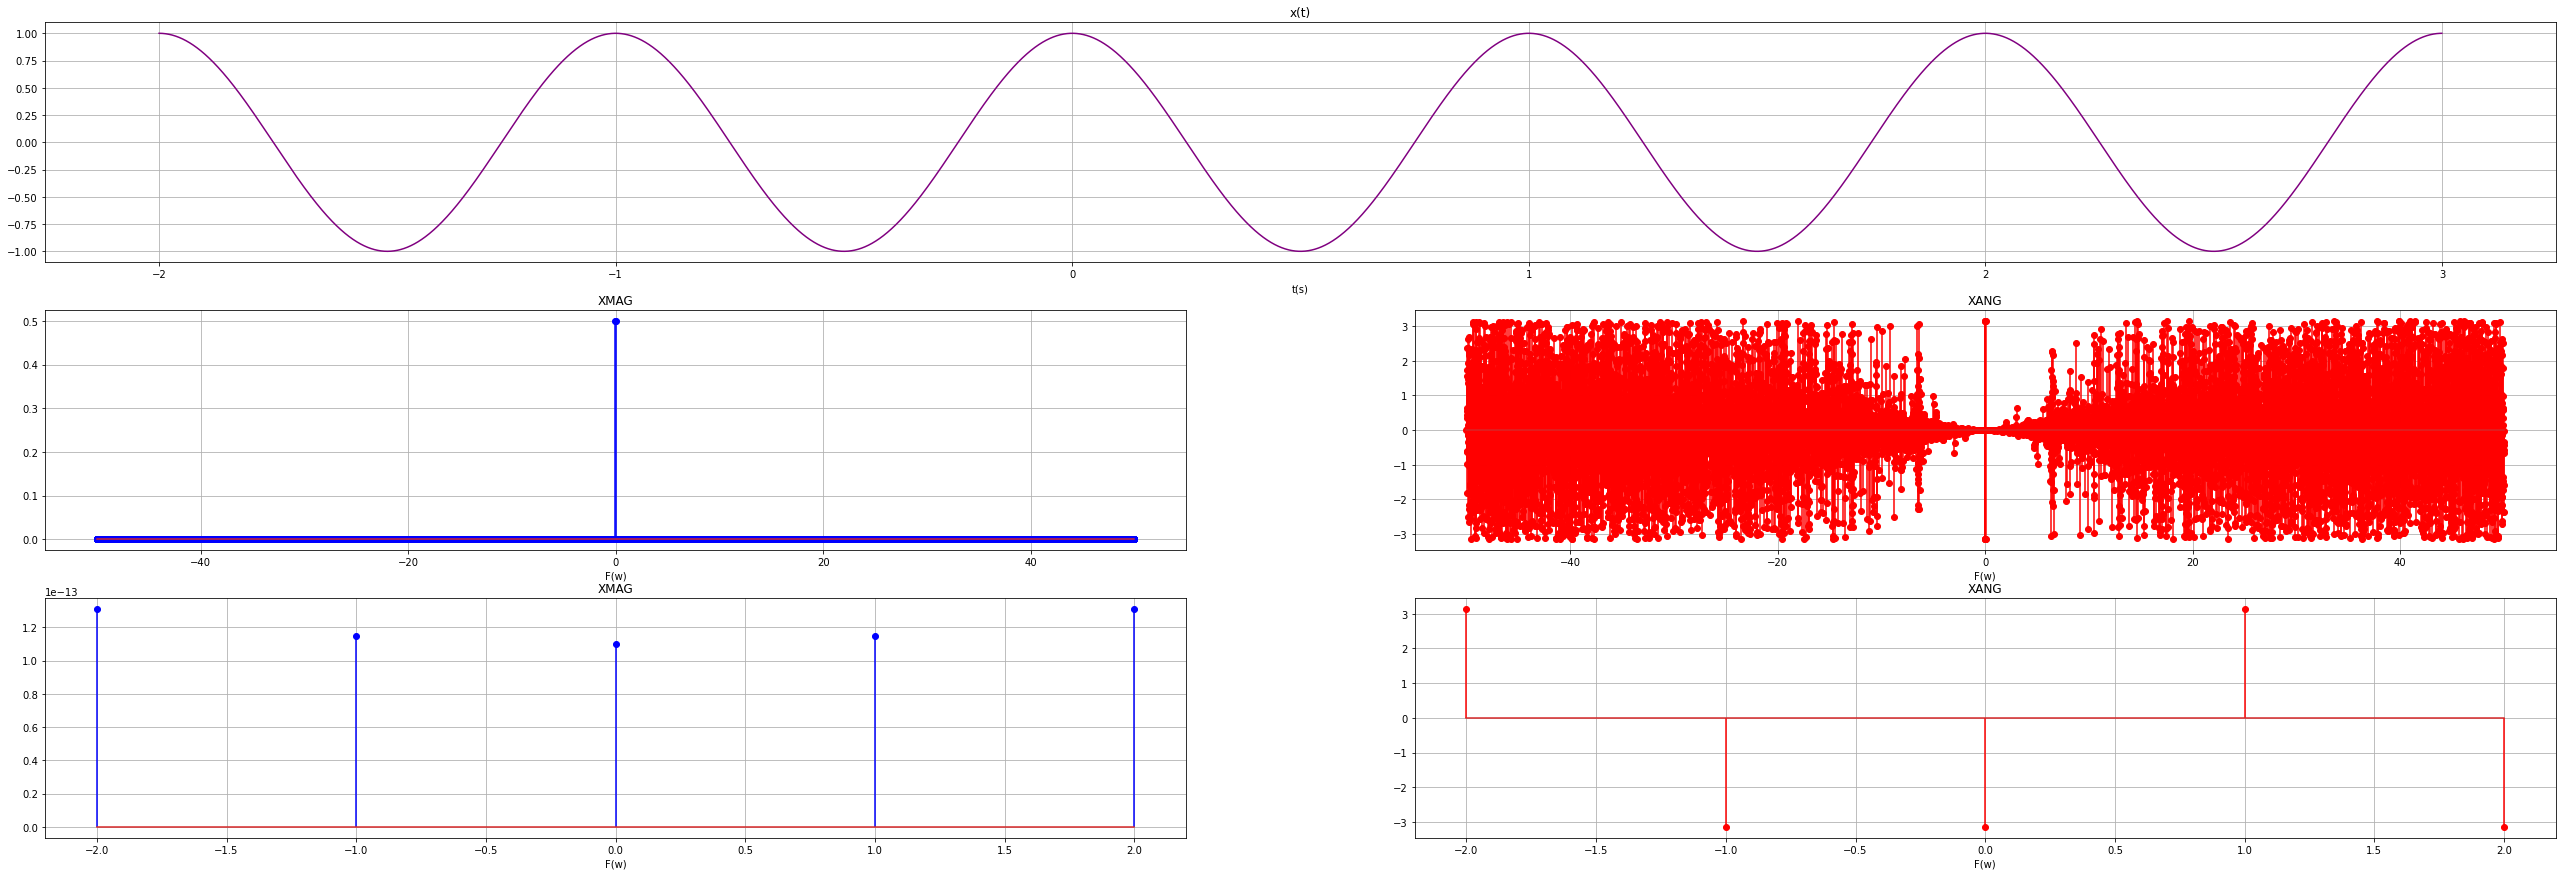
\includegraphics[width = 7in]{/home/zachariahmus/Documents/Code_Projects/ECE351/ECE351/Lab9/100.png}
\end{center}

\begin{center}
	\subsection*{fs=1000}
	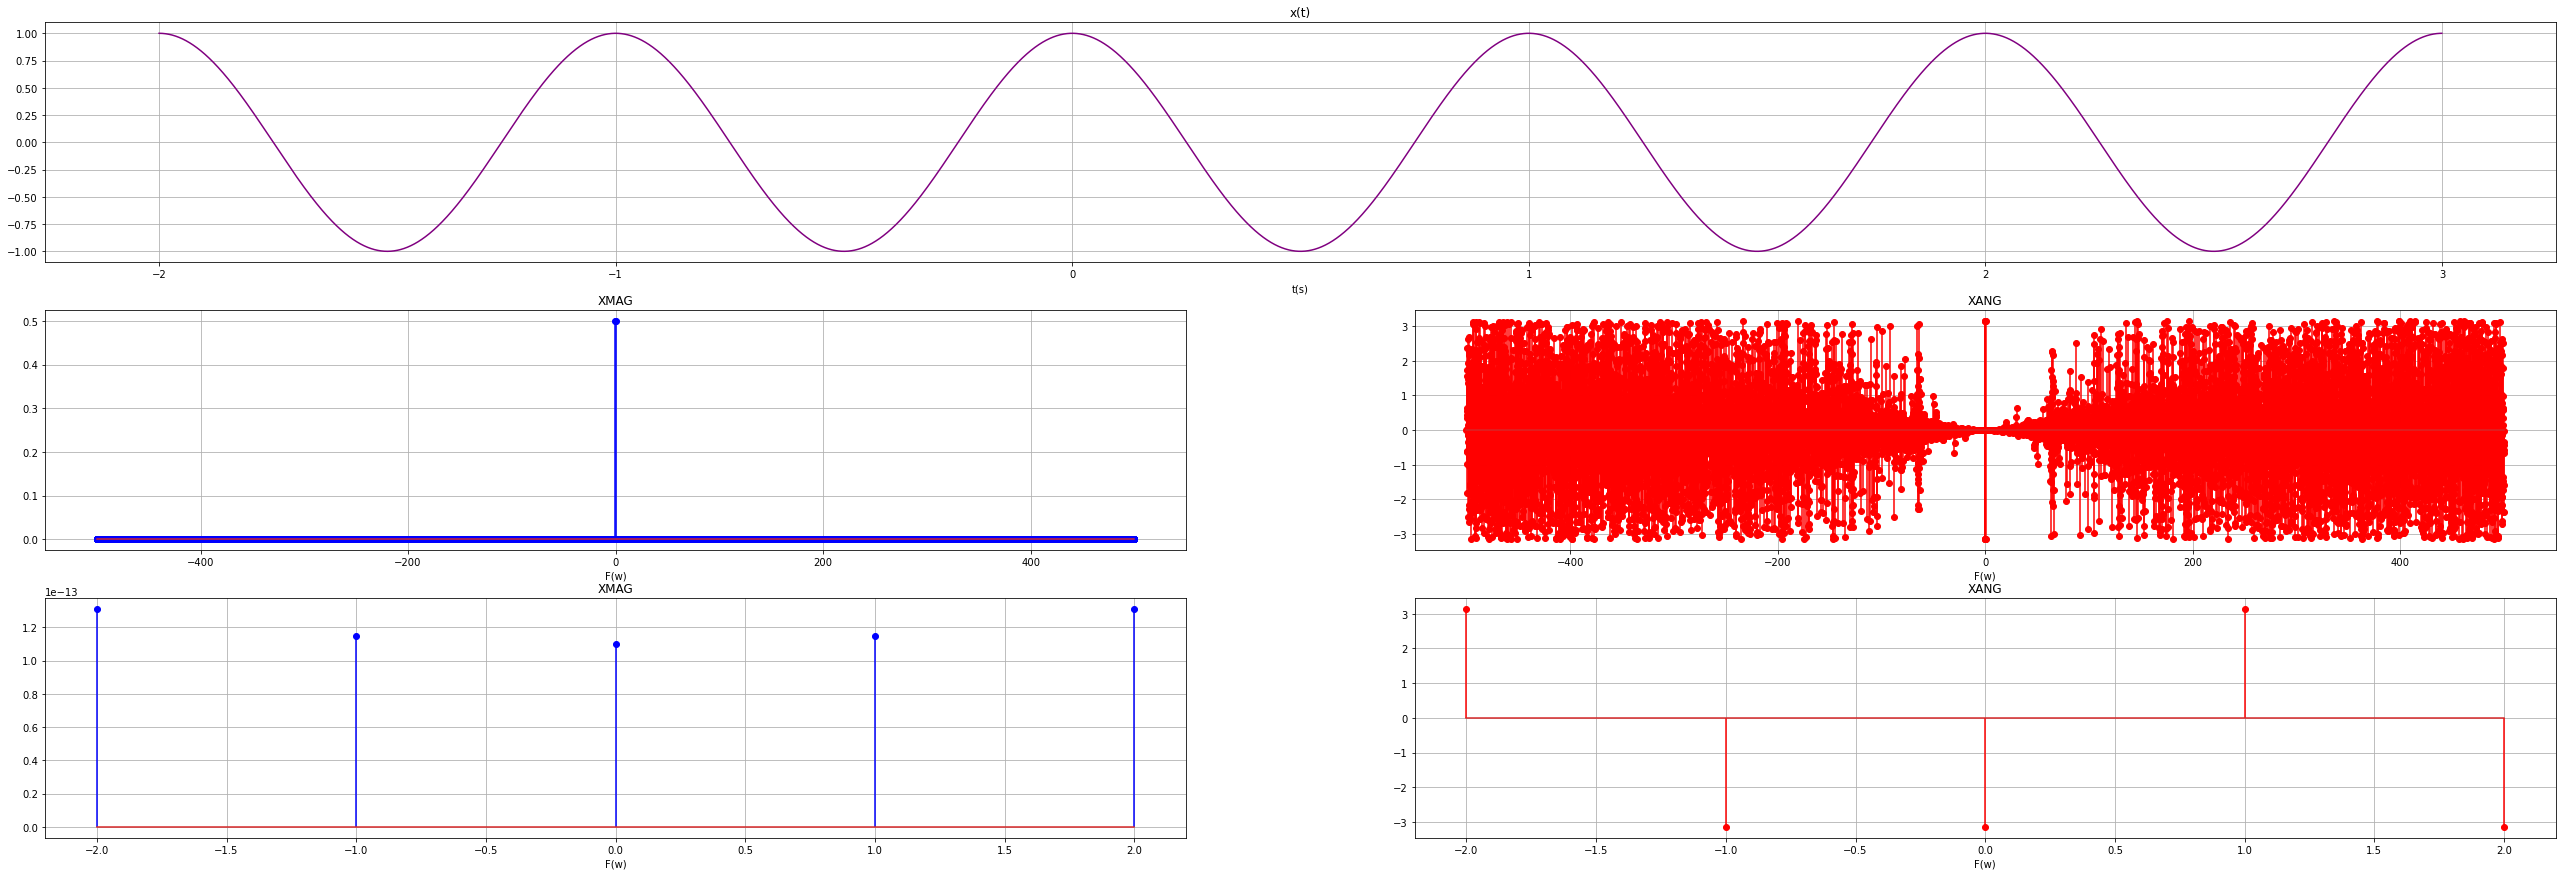
\includegraphics[width = 7in]{/home/zachariahmus/Documents/Code_Projects/ECE351/ECE351/Lab9/1000.png}
\end{center}

\begin{center}
	\subsection*{fs=10000}
	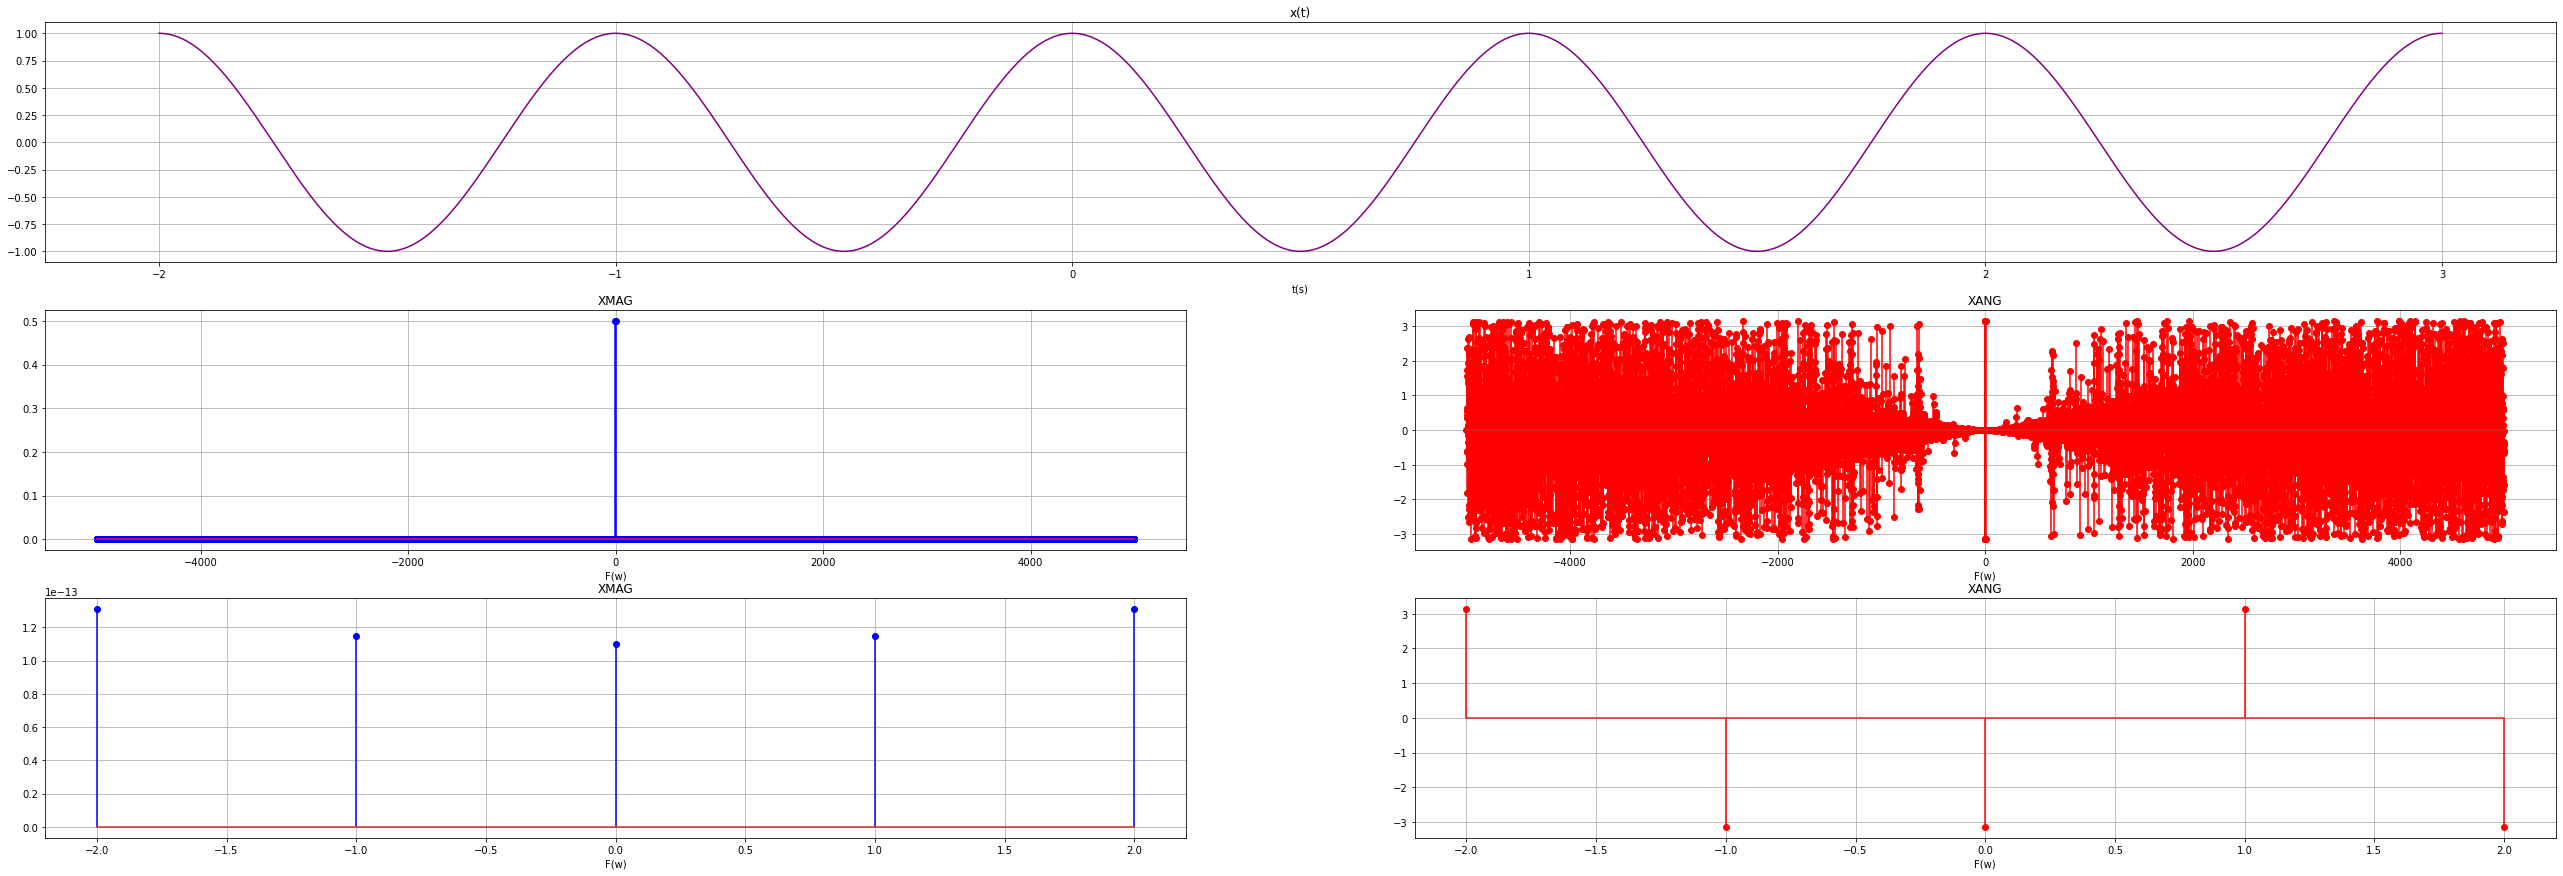
\includegraphics[width = 7in]{/home/zachariahmus/Documents/Code_Projects/ECE351/ECE351/Lab9/10000.png}
\end{center}

\begin{center}
	\subsection*{fs=100000}
	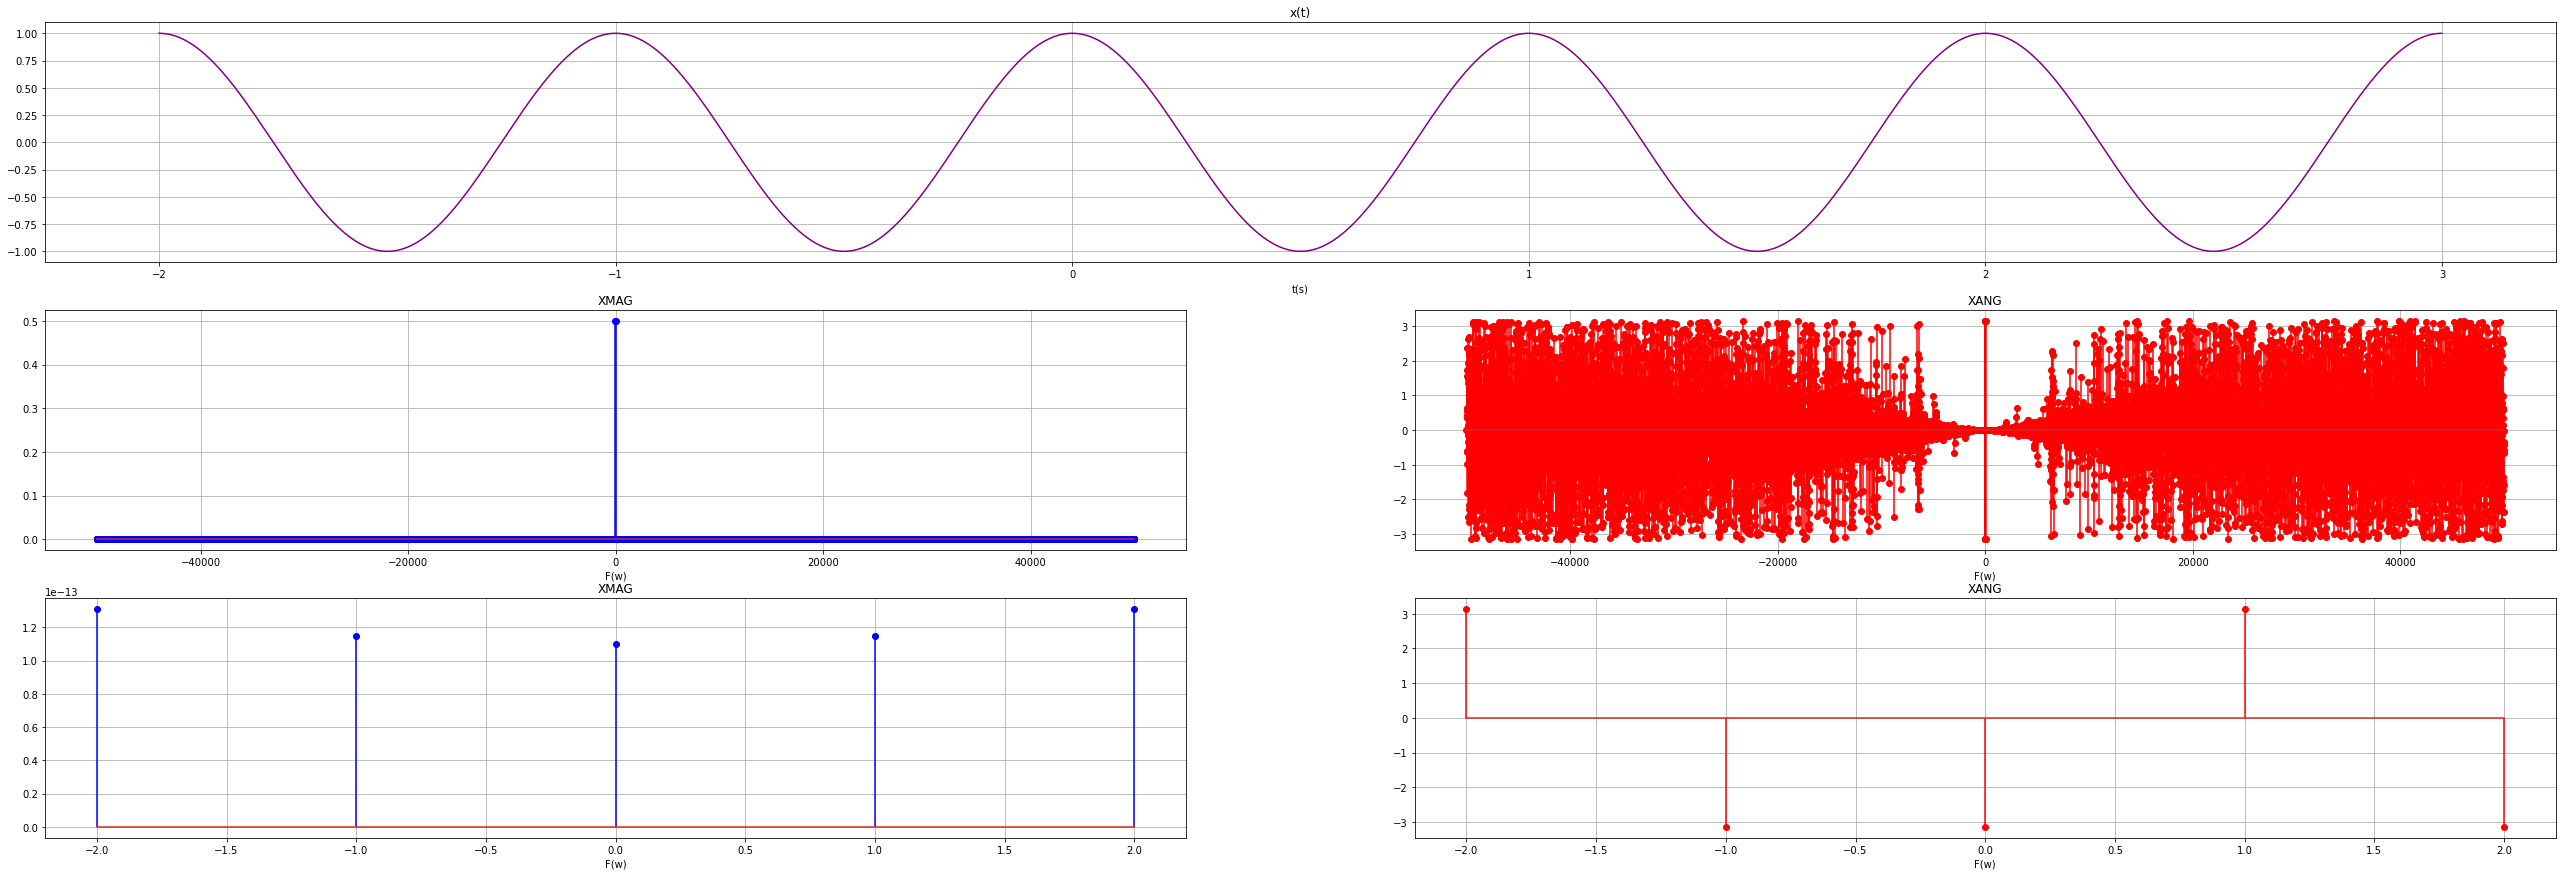
\includegraphics[width = 7in]{/home/zachariahmus/Documents/Code_Projects/ECE351/ECE351/Lab9/100000.png}
\end{center}
2. What difference does eliminating the small phase magnitudes make?\vspace*{12pt}

3. Verify your results from Tasks 1 and 2 using the Fourier transforms of cosine and sine.
Explain why your results are correct. You will need the transforms in terms of Hz, not rad/s.
For example, the Fourier transform of cosine (in Hz) is:
$$F {cos (2\pi f_0t)} = \frac{1}{2} [\delta (f - f_0) + \delta (f + f0)]$$
\vspace*{12pt}
If we look at the graph of the zoomed in magnitude plot, we will see there are two stems equidistant from the origin. This would indicate that the Fourier transform only has magnitude at two points, which would be shown by a transform consisting of just two delta functions. The graph of the transform matches the transform function, thus the results must be valid. 

4. Leave any feedback on the clarity of lab tasks, expectations, and deliverables.


\section*{Conclusion}
In this lab we were able to graph and characterize the transfer functions given to us, both how thy effect the magnitude of the incoming signal and the angle shift it enacts on it. This can be seen as potentially useful for analyzing filters and how they effect signals and what will be left afterward more easily than using just the time domain functions and graphs. 

	
\end{document}
